
In this chapter we present our main contribution,
a \textit{design pattern} for building query processing systems with the goal of evolving query processing
system architectures from monolithic and static to modular and flexible.

Traditional static query processing systems are not able to cater to the needs of modern applications in which users and
data are geo-distributed across the globe.
Our vision is to enable query processing systems that are designed and deployed on a case-by-case basis,
with the workload characteristics, data and access distribution patterns, and requirements of specific applications in
mind.

As a first step towards this vision, we focus on the \textit{mechanisms} required for enabling a flexible and configurable
query processing system architecture.

The design pattern that we propose is based on the following objectives:
\begin{itemize}
  \item \textbf{Decoupling between storage and query processing architecture.}
  The design pattern should be based on architecture, mechanism or interface of a specific data storage tier.
  Instead, it should enable query processing system to work as middleware systems on top of existing database systems.

  \item \textbf{Independence from corpus partitioning and distribution schemes.}
  The design pattern should not be based on specific a partitioning and distribution scheme for the corpus,
  but rather enable the construction of query processing systems compatible with multiple different
  data partitioning or distribution schemes.

  \item \textbf{Tunability.}
  The query processing should be able to be configured on the following dimensions:
  \begin{itemize}
    \item Index and view materialization:
    The query processing system should enable database to create secondary indexes and materialized views.
    Additionally, the index data structure used for indexes should be configurable.
    \item Caching:
    Similarly, the use of caches should be configuration-based.
    \item State maintenance scheme:
    The mode (synchronous or asynchronous) of incrementally applying corpus update to indexes and materialized views,
    should be configurable in a per index/view basis.
    \item State partitioning scheme:
    Similarly, the partitioning scheme used for secondary indexes and materialized views should be configurable in a per
    index/view basis.
  \end{itemize}

  \item \textbf{Flexible state and computation placement.}
  The design pattern should enable fine-grained control over the placement of the query processing system's derived state
  and computations.

\end{itemize}

\section{Overview: composable query processing system architecture}

The key idea for achieving the objectives described above is \textit{assembly-based modularity}
\cite{leclercq:dream, bouget:pleiades}.
A query processing system is constructed by interconnecting composable building blocks
that encapsulate derived state structures, such as indexes, materialized views, and caches,
as well as relational operators such as filters, aggregations, and joins.
In that way, configuration choices, such as index and view materialization, cache, and derived state partitioning,
translate to \textit{composition choices}: which building blocks are used and how they are interconnected.
For example, adding a caching layer to an existing query processing system can be done by extending an existing
architecture with additional ``caching'' building blocks.

Moreover, the query processing architecture's building blocks separate interface from implementation.
Because the query processing system's components communicate through well-defined interfaces,
they can be flexibly placed across the system infrastructure.
As a result, a given query processing system architecture can support multiple different component placement schemes.

\bigskip
\noindent
This design pattern defines a \textbf{modular} and \textbf{composable} component-based query processing system
architecture.
The principal element of this architecture, is its building block, which we term Query Processing Unit (QPU).

A QPU is a \textit{system component} that combines properties of a streaming operator and a microservice.
Similarly to a streaming operator, a QPU receives one or more input streams, performs a computation over these streams,
and emits an output stream.
Similarly to a microservice, a QPU provides its functionality by exposing an interface for receiving requests
(called \textit{query requests})
and can interoperate with other QPUs by sending query requests to them.
The response to query request is a stream:
every input stream that one QPU $A$ receives is the output stream of another QPU $B$, and is the response to a query request
that $A$ has sent to $B$.

\medskip
\noindent
A query processing unit can encapsulate a \textit{relational operator}.
For example, a ``join operator'' QPU receives input streams that represent the tables to be joined,
and emits an output stream that represents the results of the join operation on these tables.

Moreover, a QPU can encapsulate a \textit{derived state structure}, such as an index, a materialized view, or a cache.
For example, a ``secondary index'' QPU receives an input stream that represents notifications for updates to that table
at the corpus.
It maintains a secondary index data structure, which it stores as internal state.
When it receives a query request, it reads from its internal state and emits the result as an output stream.

Finally, a QPU can encapsulate a responsible for managing access to components of the query processing system, such as
a partition or replica manager, or a load balancer.
For example ``partition manager'' QPU, responsible for managing access to the partitions of a partitioned secondary index
(each index partition being encapsulated by a QPU), sends query requests to the appropriate index partitions for a given
query, and merges the resulting streams.

Our key insight is that all three of the described QPU types --- relational operators, derived state, and routing operators ---
can be generalized to a system component with common semantics, and thus can be composed in order to implement higher-level
query processing computations.

\medskip
\noindent
QPUs are organized in a directed acyclic graph.
The edges of the graph represent potential query request - response steam relations.
For example, an edge from a QPU $A$ to $B$ indicates that $A$ can send query requests to
--- and therefore establish input streams from --- $B$.
We call $B$ a \textit{downstream connection} of $A$, and a query request sent from $A$ to $B$ a \textit{downstream query}.
Base data are the leaves of the graph (nodes with only incoming edges),
and client queries enter the graph through its root nodes (nodes with outgoing edges).

When a QPU receives a query, it can either process it by reading from its internal state, or establish input streams
by sending query requests to its some of its downstream connections and produce query results by performing a
computation over these streams,
or a combination of the two.
As each QPU send query requests to its downstream connections,
this process is repeated at each QPU that receives a query request.
In that way, a client query results to query requests flowing downwards through the query processing system's QPU graph,
defining a \textit{query execution sub-graph}.
Query result stream flow upwards through the edge of this sub-graph.


\section{Query processing unit: a building block for composable query processing architectures}

\subsection{The Query Processing Unit component model}

The key requirement for the query processing unit is \textit{composability}:
QPUs should be able to be interconnected in various topologies,
and to interoperate in the execution of query processing tasks.

To achieve this, we define a common set of properties that every query processing unit should conform to.
This properties include the QPU's interface for receiving query requests, and the query request - response stream semantics.
We call this set of properties the query processing unit \textit{component model} (QPU model for short).
Using object-oriented programming terminology, the QPU model can be viewed as an \textit{abstract class}
that defines a set of method signatures, but not their implementation.
Implementations of the QPU model define \textit{QPU classes} with specific functionalities, for example
filter, join or materialized view QPU classes.
Using the object-oriented programming analogy, QPU classes can be viewed as classes that implement the QPU
abstract class.
Finally, specific \textit{QPU instances} can be viewed as objects of a specific QPU class, for example a secondary
index QPU for the attribute $predominantColor$ of the table $photoAlbum$.
According to the proposed design pattern, query processing systems are composed of QPU instances.

In the rest of this thesis we use the terms query processing unit, QPU, and unit interchangeably to refer to QPU instances.

\bigskip
\noindent
In this section we present an overview of the QPU model, with the goal of introducing the main concepts.
In section~\ref{ref:specification} we present the detailed specification of the QPU model.

The query processing unit component model defines a \textit{system component} with the following properties:

\begin{figure}[t]
  \centering
    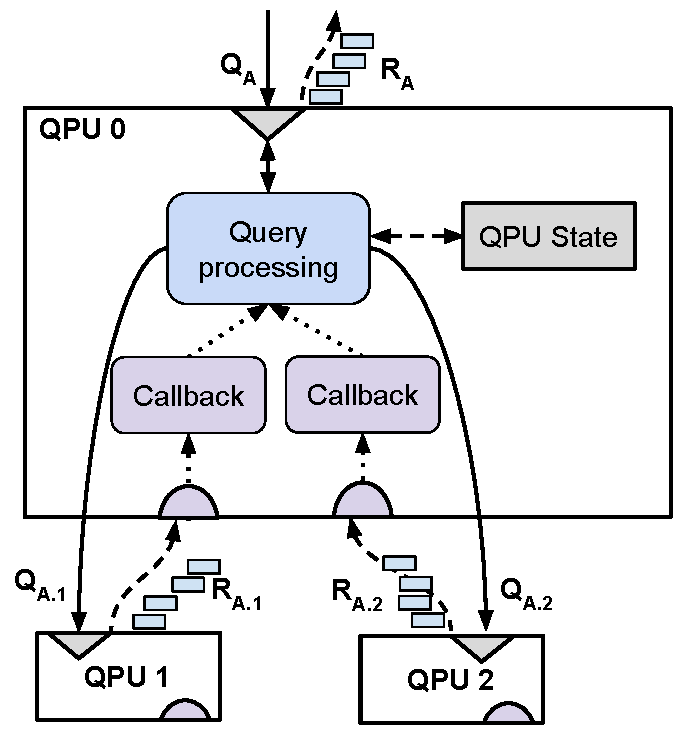
\includegraphics[width=0.5\textwidth]{./figures/design_pattern/qpu_abstraction.pdf}
  \caption{A conceptual depiction the QPU model.}
  \label{fig:qpu_abstraction}
\end{figure}

\medskip
\noindent
\textbf{Query interface.}
Query processing units expose an interface for receiving query requests.
This interface is common among all QPU classes.
As a result, a QPU can send query requests to other QPUs, regardless of their class.
This is the mechanism with which QPUs interoperate to perform query processing tasks,
and forms the basis of the query processing system's computation model (section~\ref{sec:computation_model}).

However different QPUs may be able to process only a subset of the queries that can be expressed by the interface's query
language.
For example, a QPU may only serve queries about a specific database table.
We call the set of queries that a unit can process its \textit{query processing capabilities}.

The QPU's query interface has \textit{streaming semantics}.
An invocation of the query interface initiates a stream between the QPU that sent the query request and the one that
received it;
the results of the query are sent as records through that stream.

We present the query interface in more detail in section \ref{ref:query_interface}.

\medskip
\noindent
\textbf{State.}
Each QPU maintains \textit{internal} state, that is accessible only by that QPU.

We distinguish the QPU state in three parts according to its functionality.
Each query processing unit maintains \textit{configuration state} that represents the query processing unit's
configuration parameters.
Moreover, QPUs that have downstream connections maintain information about these connections, which is
used for generating downstream query requests.
We call this part of the state \textit{local graph view}.
Finally, query processing units that implement derived state structures and QPUs that store intermediate query processing
results, for example in streaming join computations, maintain \textit{query processing state}.

\medskip
\noindent
\textbf{Initialization, query processing, and input stream callback function.}
The functionality of a query processing unit can be modeled using three functions:
\begin{itemize}
  \item The \textit{initialization function} (section~\ref{sec:initialization_func}), which is executed when the QPU is
  initialized.

  \item The \textit{query processing function} (section~\ref{sec:query_processing_func}), which is executed for each
  query request received by the QPU, and is responsible for processing the query and sending results to the response stream.

  \item The \textit{input stream callback function} (section~\ref{sec:callback_func}), which is executed for each record
  received through an input stream.

\end{itemize}

The QPU model defines the signatures of these functions, but a specific implementation.
Each QPU class provides implementations for these functions.

\bigskip

A conceptual depiction of the query processing unit model is shown in Figure~\ref{fig:qpu_abstraction}.
When the QPU's query API is called, an output stream ($R_A$) is established between the unit and the sender,
and the unit's query processing function is invoked for the given query.
The query processing function can read the QPU's state, and can perform downstream queries to other units.
For each downstream query, a corresponding stream is established ($Q_{A.1}$ and $Q_{A.2}$).
When a record is received from one of the streams, the QPU's callback function is invoked.
Each invocation of the callback function processes a received record, and returns the result to the query processing
function.
Upon receiving a result from a callback function,
the query processing function can potentially write to the QPU's state and/or emit a record to the output stream.


\subsection{Query Processing Unit component model specification}
\label{ref:specification}

In this section we present the detailed specification of the query processing unit component model.

\subsubsection{Query interface}
\label{ref:query_interface}
% we first present a high level overview of the QPU model's interface, and then describe each of its elements in more detail.

Query processing units expose an interface for receiving query requests:

\begin{displaymath}
  Query(QueryRequest) \rightarrow QueryResponse
\end{displaymath}

\begin{itemize}
  \item $QueryRequest$ specifies a predicate on the data items' \textit{attributes}, and a \textit{time interval}.

  \item $QueryResponse$ is a stream containing the query's results.
\end{itemize}

\noindent
\textbf{Query response}.

\noindent
$QueryResponse$ is a stream with the following structure:
\[
  QueryResponse = [StreamRecord]
\]
where
\[
  StreamRecord =
\]
\[
  (DataItemID,~[(AttributeName,~AttributeValue_{old},~AttributeValue_{new})],~Timestamp)
\]

\noindent
A $StreamRecord$ can represent two types of information:
\begin{itemize}
  \begin{sloppypar}
  \item An \textbf{update event} for a modification of a data item (a creation, modification, or deletion
  of a data item).
  In this case, the $StreamRecord$:
  \[
  (DataItemID,~[(AttributeName,~AttributeValue_{old},~AttributeValue_{new})],~Timestamp)
  \]
  represents an update to the the data item $DataItemID$, with timestamp $Timestamp$;
  Each elements of $[(AttributeName$, $AttributeValue_{old}$, $AttributeValue_{new})]$ indicates that
  the update modified the value of attribute $AttributeName$ from $AttributeValue_{old}$ to $AttributeValue_{new}$.
  \end{sloppypar}

  \begin{sloppypar}
  \item The \textbf{state of a data item}.
  In this case, $StreamRecord$:
  \[
  (DataItemID,~[(AttributeName,~AttributeValue_{old},~AttributeValue_{new})],~Timestamp)
  \]
  encodes that the data item $DataItemID$ at timestamp $Timestamp$;
  Each elements of $[(AttributeName$, $AttributeValue_{old}$, $AttributeValue_{new})]$ indicates that
  the data item is associated with an attribute $AttributeName$ with the value $AttributeValue_{new}$
  ($AttributeValue_{new}$ is ignored).
  \end{sloppypar}
\end{itemize}

\medskip
\noindent
\textbf{The query request's time interval.}

\noindent
Given a $QueryRequest$ that specifies a projection $Proj$,
an attribute predicate $Pred$
and a time interval $T$ $=$ $[t_1, t_2)$:
\begin{itemize}

  \item if \textbf{$t_1$ $<$ $t_2$},
  then $QueryResponse$ contains an update event for each update $u$ with $t_1$ $\leq$ $timestamp$ $<$ $t_2$,
  for which one of the following is true:
  \begin{itemize}
    \item $u$ creates a data item $d$, and $d$'s attributes satisfy $Pred$.

    \item $u$ deletes a data item $d$, and $d$'s attributes satisfy $Pred$ before deletion.

    \item $u$ modifies a data item $d$, and:
    \begin{itemize}
      \item The state of $d$ before $u$ is applied, after, or both satisfies $Pred$, and
      \item $Proj$ contains one of the modified attributes.
    \end{itemize}

    This covers the following cases:
    \begin{itemize}
      \item An update modifies a data item so that its state before the update is applied does not satisfy $Pred$,
      but its state after the update is applied satisfies $Pred$.
      In that case, the data item needs to be added to the posting list of an index entry, or to the results of a
      materialized view.

      \item An update modifies a data item so that its state before the update is applied satisfies $Pred$,
      but its state after the update is applied does not satisfy $Pred$.
      In that case, the data item needs to be removed from the posting list of an index entry, or to the results of a
      materialized view.

      \item An update modifies a data item, both its state before the update is applied and after satisfies $Pred$,
      and the data item's state stored as part of the index entry of the materialized view (because of $Proj$) is modified.
    \end{itemize}
  \end{itemize}
  We term this type of query \textit{an interval query}.

  By using a upper bound ($t_2$) in the future (a timestamp that the system has not yet reached),
  an interval query can continue receiving future updates that satisfy $Pred$.
  This provides a mechanism for \textit{subscribing to notification for updates}.

  \item If \textbf{$t_1$ $=$ $t_2$ = $t$},
  then the query is performed on a \textit{snapshot} of the corpus that contains the effects of all updates with
  $timestamp$ $<$ $t$.
  For each data item $d$ that satisfies $Pred$, $QueryResponse$ contains a $StreamRecord$ that encodes the state of $d$
  at timestamp $t$.
  We term this type of query a \textit{snapshot query}.

\end{itemize}

% By returning the latest update before a given timestamp $t$,
% a snapshot query effectively returns the \textit{state} of each data item that satisfies $Pred$ at $t$.
% Therefore,
% A snapshot query refers to a \textit{snapshot} of the corpus that contains the effects of all update with $timestamp$ $<$ $t$.

% An interval query returns may returns any update with timestamp within the specified time interval which modifies a
% data item so that either its old state value before applying the update or the new value after  is starts or it stops
% satisfying $Pred$.

\medskip
\noindent
\textbf{Response stream mode.}

\noindent
The query response stream can be either synchronous or asynchronous.
In a synchronous stream, the sender blocks until the stream records has been received and processed by the receiver.

\medskip
\noindent
\textbf{Query Language.}

\noindent
% https://documentation.basis.com/BASISHelp/WebHelp/usr2/sql_grammar.htm
% http://www.h2database.com/html/grammar.html#expressionz
The query processing unit interface support a query language with an SQL-like syntax.
The query language supports point and range queries, logical operators, aggregation functions, and joins.
We argue that these is no inherent limitation in the QPU model that prevents it from supporting a more complex
query language (for example supporting nested queries).
However, we consider additional functionalities to be out of the scope of this work.
We believe this query language can effectively demonstrate that the QPU model can be used as building
block for constructing fully-functional query processing systems.

\medskip
\noindent
The QPU model's query language has following syntax:

{\obeylines\obeyspaces
\texttt{
QueryRequest          ::=  SELECT SelectExpression
~~~~~~~~~~~~~~~~~~~~~~~~~~~FROM TableExpression
~~~~~~~~~~~~~~~~~~~~~~~~~~~WHERE PredicateExpression
~~~~~~~~~~~~~~~~~~~~~~~~~~~TIMESTAMP TimestampExpression \todo{the timestamp can be just another attribute, but I think we need to have it separate for emphasis}
~~~~~~~~~~~~~~~~~~~~~~~~~~~[ GROUP BY attributeName ]
% ~~~~~~~~~~~~~~~~~~~~~~~~~~~[ ORDER BY OrderByExpression \{ ASC | DESC \} ]
~~~~~~~~~~~~~~~~~~~~~~~~~~~\{ SYNC | ASYNC \}
}}

{\obeylines\obeyspaces
\texttt{
SelectExpression      ::=  ALL
~~~~~~~~~~~~~~~~~~~~~~~~~~~SelectExpressionItem , SelectExpression |
~~~~~~~~~~~~~~~~~~~~~~~~~~~SelectExpressionItem
}}

{\obeylines\obeyspaces
\texttt{
SelectExpressionItem  ::=  SUM(attributeName) | AVG(attributeName) |
~~~~~~~~~~~~~~~~~~~~~~~~~~~MAX(attributeName) | MIN(attributeName) |
~~~~~~~~~~~~~~~~~~~~~~~~~~~attributeName
}}

{\obeylines\obeyspaces
\texttt{
TableExpression       ::=  tableName JoinType tableName On tableName.attributeName = tableName.attributeName |
~~~~~~~~~~~~~~~~~~~~~~~~~~~tableName
}}

{\obeylines\obeyspaces
\texttt{
JoinType              ::=  \{ INNER | \{ LEFT | RIGHT \} OUTER \} JOIN
}}

{\obeylines\obeyspaces
\texttt{
PredicateExpression   ::=  PredicateExpression OR PredicateExpression |
~~~~~~~~~~~~~~~~~~~~~~~~~~~PredicateExpression AND PredicateExpression |
~~~~~~~~~~~~~~~~~~~~~~~~~~~NOT PredicateExpression |
~~~~~~~~~~~~~~~~~~~~~~~~~~~Term Op Term
}}

{\obeylines\obeyspaces
\texttt{
Term                  ::=  attributeName | Value
}}

{\obeylines\obeyspaces
\texttt{
Op                    ::= > | >= | < | <= | = | !=
}}

{\obeylines\obeyspaces
\texttt{
Value                 ::= stringValue | floatValue | intValue |
~~~~~~~~~~~~~~~~~~~~~~~~~~dateTimeValue | timestampValue
}}

% {\obeylines\obeyspaces
% \texttt{
% OrderByExpression     ::= attributeName , OrderByExpression |
% ~~~~~~~~~~~~~~~~~~~~~~~~~~attributeName
% }}
{\obeylines\obeyspaces
\texttt{
TimestampExpression   ::= FROM TimestampTerm [ TO TimestampTerm ]
}}

{\obeylines\obeyspaces
\texttt{
TimestampTerm         ::= SYSTEM START | LATEST | timestampValue
}}

~ \bigskip

\noindent
In practice, each QPU instance can only process a subset of the queries that can be expressed by this query language,
according to the functionality supported by its class.
For example, a QPU class that implements a join operator can perform join over two input streams,
but not evaluate a $PredicateExpression$, or perform an $SUM$ on an attribute of the join result.
This can be achieved by connecting ``join'', ``filter'', and ``aggregator'' QPUs.
We present in detail these QPU classes in section~\ref{sec:qpu_classes},
and how they are composed to provide complex query processing functionalities in section~\ref{sec:query_processing_system}.

Moreover, instances of a certain class may support different parts of the query language according to their
configuration.
For example, two instances of a filter operator QPU class may support predicate queries for different tables.

\subsubsection{QPU State}

The query processing unit's state is divided into the following parts:

\medskip
\noindent
\textbf{Configuration state.}
Upon initialization, each QPU receives is given a set of configuration parameters.
These parameters are represented as key-value pairs.
The configuration state represents these parameters.

Configuration parameters can be divided to the following parts:
\begin{itemize}
  \item Topology configuration.
  This part of the configuration consists of the endpoints of the QPU's downstream connections in the QPU graph.

  \item Class-specific configuration.
  The part of the configuration specifies parameters such as cache size or the definition of a materialized view.
\end{itemize}

% \begin{lstlisting}[caption={Pseudocode for the QPU's configuration state},captionpos=b,label={lst:qpuconfigstate}]
% class ConfigurationState
%   function GetConfigParameter(Key) ConfigParameterValue
% \end{lstlisting}

\medskip
\noindent
\textbf{Local graph view.}
For each of its downstream connections, a query processing unit maintains a data structure that represents the
\textit{set of queries that this connection can process}, which we term \textit{query processing capabilities}.
It the query processing capabilities of its neighbors in order to: (1) validate if it can process a given
query, and (2) generate downstream queries for a given query.

The data structures for the query processing capabilities of a QPU's downstream connections compose it local graph view
state.

In section~\ref{sec:qpc_tree} we present query processing capabilities data structure as well as its use in detail.

\medskip
\noindent
\textbf{Query processing state.}
Query processing units that encapsulate derived state structures such as indexes, materialized views and
caches, store these data structures in the part of their state that we call \textit{query processing state}.
Additionally, streaming operator QPUs such as joins use this part of the state to store intermediate state.

We model the query processing state as set of key-value pairs, ordered by key:
\[
  (Key,~[State],)
\]
where
\[
  State = (DataItemID,~[(AttributeName,~AttributeValue)],~Timestamp)
\]
% and
% \[
%   Timestamp_S := \{t \in [DataItemState] : t > Timestamp_U~\forall~Timestamp_U \in [DataItemState] \}
% \]

% The timestamp $Timestamp_S$ of an entry of the query processing state is the latest of the timestamps $Timestamp_U$
% contained in the entry's value.

Using pseudocode, we can represent the query processing state's API as follows:

\begin{lstlisting}[caption={Pseudocode for the QPU's query processing state},captionpos=b,label={lst:qpustate}]

type AttributeName string

type AttributeValue union {
  string
  float
  int
  dateTime
  timestamp
}

type State {
  dataItemID  string
  attributes  [(AttributeName, AttributeValue)]
  ts          timestamp
}

class QueryProcessingState
  function Put(Key, State)
  function Get(Key_low, Key_high, Timestamp_low, Timestamp_high) [(Key, [State])]
\end{lstlisting}

\begin{itemize}
  \item $Put$ modifies the value of the query processing state's entry for the given key.
  It can be used with a non-existing key to create a new entry.

  \item $Get$ retrieves the query processing state entries with $Key_low$ $<$ $key$ $\leq$ $Key_high$.
  For each entry, the updates with $Timestamp_low$ $<$ $Timestamp$ $\leq$ $Timestamp_high$ retrieved.
\end{itemize}

Essentially, the QPU's query processing state is versioned.
In that way, QPU's can process queries about any timestamp that they have received updates for.


\subsubsection{Initialization function}
\label{sec:initialization_func}

Each QPU invokes an initialization function when it starts its execution.

\begin{lstlisting}[caption={Initialization function signature},captionpos=b,label={lst:init_func}]
type DownstreamConnection {
  endpoint sting
  capabilities QPCapabilities
}

function Init(QPState, [DownstreamConn])
\end{lstlisting}

\noindent
Listing~\ref{lst:init_func} shows the initialization function's signature.
$ProcessQuery$ receives as arguments:
\begin{itemize}
  \item $QPState$, which is a handler that enables $Init$ to read from and write to QPU's query processing state.

  \item A list of $DownstreamConn$, each consisting of the endpoint of a downstream connection and a data structure
  representing the connection's query processing capabilities (section~\ref{sec:qpc_tree}).
  $Init$ can therefore send downstream query requests.
\end{itemize}


\subsubsection{Query processing function}
\label{sec:query_processing_func}

The query processing function is responsible for processing a given query and emitting the results to the output stream.

For each query $q$ being processing, the QPU initiates an output stream, $R_q$,
and executed an instance of the query processing function, $QPF_q$.
$QPF_q$ is responsible for emitting records to $R_q$.
Moreover, if $QPF_q$ initiates input streams $I_{q-1}$, $I_{q-2}$, ..., then $QPF_q$ is responsible for handing the return
values of callback functions for records received through $I_{q-i}$.

\begin{lstlisting}[caption={Query processing function signature},captionpos=b,label={lst:query_processing_func}]
function ProcessQuery(QueryRequest, QPState, [DownstreamConn],
                      ResponseStream)
\end{lstlisting}

\noindent
\begin{sloppypar}
Listing~\ref{lst:query_processing_func} shows the query processing function's signature.
In addition to $QPState$ and $[DownstreamConn]$, $ProcessQuery$ receives:
\end{sloppypar}
\begin{itemize}
  \item $QueryRequest$, which represents the received query request.

  \item $ResponseStream$, a handler it can use to emit result to the output stream.

\end{itemize}

An instance of the query processing function is executed for each received query request,
therefore query processing unit can run multiple instances of the query processing function in parallel.

\subsubsection{Input stream callback function}
\label{sec:callback_func}

The input stream callback function is responsible for processing a record received through an input stream.
The callback function can read from and write to the query processing unit state,
and a (potentially empty) list of $StreamRecord$ to the query processing function.

\begin{lstlisting}[caption={Input stream callback function signature},captionpos=b,label={lst:callback_func}]
function ProcessInputRecord(StreamRecord, QueryRequest, QPState)
          returns [StreamRecord]
\end{lstlisting}

\noindent
Listing~\ref{lst:callback_func} shows the query processing function's signature.

An instance of the callback function is executed for each record received through an input stream.

\subsection{Stream semantics}

In this section we describe more detail the semantics of the stream connections between query processing units.

\medskip
\noindent
Apart from \textit{data records} (updates), \textit{control records} can also be sent through a stream.
Although ata records can be sent only in one direction (``upstream''), control records can be sent in both directions.
Types of control records include acknowledgements, heartbeats, and re-send requests.
A re-send records requests for a data record to be re-send.

\medskip
\noindent
Sending a data record can be either \textit{synchronous} or \textit{asynchronous}.
A synchronous send operation blocks until an acknowledgement for the data record is received.

\medskip
\noindent
Finally, we assume that stream connections do not drop, re-order, of duplicate messages;
however messages may be arbitrarily delayed.
These guarantees are not based on assumptions about the transport layer, but as we discuss in In chapter~\ref{ch:evaluation}
are implemented by query processing units on top of potentially unreliable connections.


\subsection{Query processing unit consistency semantics}

//// Outline ////

\noindent
Internal consistency

\noindent
We refer to a derived state QPU as \textit{internally consistent} in time $t$ if its query processing state
reflects all updates with timestamp $\leq$ $t$ and no updates with timestamp $>$ $t$.

Since the query processing storage is multi-versioned, with each version corresponding to an update,
the query processing state with version $T$ $\in$ $StateVersions$
\[
  \nexists~T' \in StateVersions : T' > T \land T < t
\]
by definition reflects only updates with timestamps $\leq$ $t$ and no updates timestamp $>$ $t$.
In order to guarantee that this version is internally consistent, the QPU must ensure that this version reflects
\textbf{all} updates with timestamp $\leq$ $t$.

Showing that this is ensured consists of three parts.
\begin{itemize}
  \item Updates entering the QPU graph in-order according to their timestamp.
  We can assume the interface between database and corpus driver QPU guarantees that.
  \item Updates are not reordered by the stream connections.
  This is part of our assumptions about the stream semantics.
  \item Updates are not reordered by relational operator QPUs.
  This is trivial for QPUs with a single input stream.
  We need to show that QPUs that merge more that one stream produce ordered streams ...
\end{itemize}

If these three conditions are true then each QPU receives and processes updates in order.
Therefore, is has processed an update with timestamp $t$ then it has also processed all updates with timestamp $\leq$ $t$.

\medskip
\noindent
Query consistency

\noindent
We refer to a query with time interval $[t_1, t_2)$ as \textit{consistent} if all corpus driver and derived state QPUs
that take part in its execution are internally consistent at time $t_2$.

\noindent
//// Outline ////


\subsection{QPU classes}
\label{sec:qpu_classes}

As described in the previous section, the query processing unit component model has the role of ``template'',
defining unified semantics that every QPU conforms with.
This ensures that QPU instance with different functionalities (classes) and configurations can be interconnected and
can interoperate to perform query processing tasks.

A QPU class is an \textit{instantiation} of the query processing unit model:
it defines the implementations of the \textbf{initialization}, \textbf{query processing} and \textbf{input stream callback}
functions.

In this section, we present a categorization of QPU classes according to their general characteristics,
and demonstrate some examples of QPU classes.
We present additional QPU classes in chapters~\ref{ch:case_studies}, \ref{ch:proteus}, \ref{ch:evaluation}.

We categorize QPU classes in three groups, according to their general characteristics:
\begin{itemize}
  \item \textbf{Relational operator classes}.
  Classes in this group encapsulate \textit{streaming relational operators}.
  A relational operator QPU receives one or more input data streams, and perform a transformation over these streams.
  For every record received through one of the input streams, the QPU emits zero or one record at the output stream.

  Every input stream of relational operator QPU is the output stream of another QPU, and has been establish as a response
  to a query request.

  Examples of QPU classes in this group are:
  \begin{itemize}
    \item \textbf{Filter:}
    A filter QPU receives records from an input stream, and  emits at its output those records satisfy a given condition.

    \item \textbf{Join}:
    A join QPU encapsulates a streaming join operator.
    It receives records from two or more input streams, and performs a join operation one those stream, according
    to parameters specified by a given query request.
    The join QPU initiates input streams by sending the appropriate query requests to its downstream connections,
    and emits ths join operation result as its output stream.

    \item \textbf{Aggregator classes}:
    Aggregator QPU classes encapsulate aggregation function such as count, sum, average, and min or max.
    An aggregator QPU performs a streaming aggregation over an input stream;
    It emits a record at its output stream for each input record that changes the computed aggregation value.
  \end{itemize}

  \item \textbf{Derived state classes}.
  Classes in this group encapsulate derived state structures, such as indexes, caches, and materialized views.

  This group includes the following classes:
  % QPUs of derived state classes make use of the same use of the ``query request - output stream'' semantics to implement their functionality:
  \begin{itemize}
    \item \textbf{Secondary index and Materialized view:}
    A secondary index (or materialized view) QPU receives its index or view definition as a configuration parameter.

    The QPU's initialization function establishes an input steam by sending an \textit{interval} query
    (a query without an upper bound timestamp) to its downstream connection:
    In that way, the QPU effectively \textit{subscribes to notifications} for updates to the corpus.
    For each record received through the input stream, the callback function updates the query processing state accordingly.
    When a query request is received,
    the query processing function computes the results by reading from the query processing state,
    and emits them to the output stream.

    % For simplicity we assume that a secondary index QPU maintains an index for a single attribute (and the same for materialized view QPUs respectively).
    \item \textbf{Cache:}
    When receiving a query request, a cache QPU's query processing function first determines if the query result is stored
    in the query processing state.
    If yes, the function retrieves the corresponding query results and emits them at the output stream.
    Alternatively, the query processing function sends a query request at the QPU's downstream connection,
    with the given query.
    The callback function stores each received record, and then returns it to the query processing function with emits it
    at the output stream.
    \end{itemize}

  \item \textbf{Routing classes}.
  Classes in this group encapsulate query processing functionalities that can be characterized as ``query routing''.
  This includes coordinating access to partitioned or replicated derived indexes and materialized views,
  or load balancing.

  Examples of classes in this group include:
  \begin{itemize}
    \item \textbf{Partition manager:}
    A partition manager QPU is responsible for coordinating access secondary index or materialized view partitions,
    encapsulated by the corresponding QPU classes.

    A partition manager QPU has downstream connections to a set of QPUs representing partitions.
    When a query request is received, the QPU's query processing function determines which partitions need to be contacted,
    generated the corresponding queries and sends them as downstream query requests.
    To enable this, the partition manager QPU maintains information about the partitioning scheme and the portion of
    the partitioned space that corresponds to each of its downstream connections connections at its query processing
    capabilities spaces
    The unit then merges the input streams and emits the result as its output stream.

    \item \textbf{Load balancer and replica manager:}
    QPUs of these classes have similar functionalities with the partition manager class.
    Given a query, the query processing function of a load balancer or replica manager QPU selects the most suitable
    among the QPU's downstream connections according to a certain criterion (defined by QPU's class and configuration),
    forwards the given query to that connection, and then forwards the resulting input stream to the output stream.
    \end{itemize}

  \item \textbf{Corpus driver classes}.
  Classes in this group are responsible for connecting the QPU graph with the corpus.
  QPUs of these classes do not support downstream connections to other QPUs.
  Because of their functionality, corpus driver QPUs are only used as leaves of the QPU graph.
  In fact, as we explain in section~\ref{sec:graph_topology}, every leaf node of the QPU can only be a corpus driver QPU.

  When a query request is received, the query processing function of a corpus driver QPU uses the interface and mechanisms
  of they corpus database in order to generate and emit the output stream that corresponds to the given query.
  This can include reading from the database that stores the corpus, subscribing to update notifications,
  or performing queries.

  The corpus driver classes act as a wrappers for the corpus, exposing a common interface and semantics to the
  QPU graph, independent of how the corpus is stored and accessed.
  As a result, corpus driver classes are database-specific.

  QPU-based query processing systems can be compatible with any corpus database --- or, more generally, source of updates ---
  for which there is a corresponding corpus driver class.
\end{itemize}

\subsubsection{QPU class case studies}

\textbf{Filter}

Algorithms~\ref{algo:filter_query_processing_func} and~\ref{algo:filter_algorithm_func} show the query processing and
input stream callback functions respectively for the filter QPU class using pseudocode.


\begin{algorithm}
\caption{Filter QPU class query processing function}
\label{algo:filter_query_processing_func}
\begin{algorithmic}
\Function{ProcessQuery}{queryReq, qpState, [downstreamConn], outputStream}
\State conn = get endpoint from [downstreamConn] \Comment{we assume one downstream connection}
\State inStream = forward queryReq to conn
\While{not at end of this the stream}
\State inRecord = inStream.Recv()
\State result = ProcessInputRecord(inRecord, queryReq, qpState)
\If{result is not empty}
\State outStream.Send(result)
\EndIf
\EndWhile
\EndFunction
\end{algorithmic}
\end{algorithm}

\begin{algorithm}
\caption{Filter QPU class input stream callback signature}
\label{algo:filter_algorithm_func}
\begin{algorithmic}
\Function{ProcessInputRecord}{inRecord, queryReq, qpState}
\If{inRecord satisfies queryReq}
\State \Return inRecord
\Else
\State \Return []
\EndIf
\EndFunction
\end{algorithmic}
\end{algorithm}


\bigskip
\noindent
\textbf{Secondary index}

Algorithms~\ref{algo:index_init_func}, ~\ref{algo:index_query_processing_func}, and~\ref{algo:index_callback_func}
show the initialization, query processing, and input stream callback functions respectively for the secondary index QPU
class using pseudocode.

\begin{algorithm}
\caption{Secondary index QPU class initialization function}
\label{algo:index_init_func}
\begin{algorithmic}
\Function{Init}{qpState, [downstreamConn]}
\State conn = get endpoint from [downstreamConn] \Comment{we assume one downstream connection}
\State queryReq = generate interval query
\State inStream = send queryReq to conn
\While{not at end of this the stream}
\State inRecord = inStream.Recv()
\State ProcessInputRecord(inRecord, null, qpState)
\EndWhile
\EndFunction
\end{algorithmic}
\end{algorithm}

\begin{algorithm}
\caption{Secondary index QPU class query processing function}
\label{algo:index_query_processing_func}
\begin{algorithmic}
\Function{ProcessQuery}{null, qpState, [downstreamConn], outputStream}
\State conn = GetEndpoint([downstreamConn]) \Comment{we assume one downstream connection}
\State inStream = forward queryReq to conn
\While{not at end of this the stream}
\State inRecord = inStream.Recv()
\State result = ProcessInputRecord(update)
\If{result is not empty}
\State outStream.Send(result)
\EndIf
\EndWhile
\EndFunction
\end{algorithmic}
\end{algorithm}

\begin{algorithm}
\caption{Secondary index QPU class input stream callback function}
\label{algo:index_callback_func}
\begin{algorithmic}
\Function{ProcessInputRecord}{inRecord, queryReq, qpState}
\State (dataItemID, [attributeDelta], timestamp) = parse inRecord
\For {(attrName, attrValOld, attrValNew) in [AttributeDelta]}
\If{attrValOld is not null}
\State indexTerm = build index term from attrName and attrValOld
\State postingList = qpState.Get(indexTerm, indexTerm)
\State postingList' = remove dataItemID from postingList
\State pState.Put(indexTerm, postingList')
\EndIf
\If{attrValNew is not null}
\State indexTerm = build index term from attrName and attrValNew
\State postingList = qpState.Get(indexTerm, indexTerm)
\State postingList' = add dataItemID from postingList
\State pState.Put(indexTerm, postingList')
\EndIf
\EndFor
\EndFunction
\end{algorithmic}
\end{algorithm}


\section{QPU-based query processing systems}
\label{sec:query_processing_system}

\subsection{Query processing system architecture}

\begin{figure}[t]
  \centering
    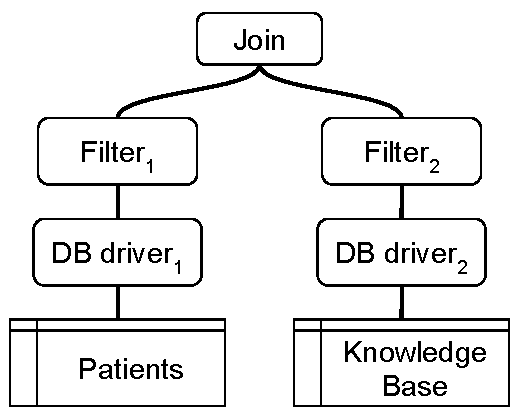
\includegraphics[width=0.4\textwidth]{./figures/design_pattern/qpu_graph_emergent_properties.pdf}
  \caption{QPU graph example}
  \label{fig:qpu_graph_emergent_properties}
\end{figure}

A \textit{QPU-based} query processing system is a directed acyclic graph (DAG) with query processing unit instances as
graph nodes.
Edges represent potential query request - response stream relations between QPUs:
a directed edge from $QPU_a$ to $QPU_b$ indicates that $QPU_a$ is able to send query requests to $QPU_b$.
A query request sent from $QPU_a$ to $QPU_b$ initiates a stream connection between $QPU_a$ and $QPU_b$;
$QPU_b$ emits query results through that stream.

The corpus is represented by the graph's leaf nodes (nodes with no outgoing connections).
Queries enter the QPU graph through root nodes (nodes with no incoming connections).

The capabilities of a QPU-based query processing system are emergent from the functionalities of the QPUs it is composed of,
as well as the graph topology.
For example, consider the QPU graph depicted in Figure~\ref{fig:qpu_graph_emergent_properties}, where:

\begin{lstlisting}[caption={Customer and Orders tables attributes},captionpos=b,]
Table Customers(CustomerID, Email, Address)
Table Orders(OrderID, CustomerID, OrderStatus, OrderDate)
\end{lstlisting}

\begin{itemize}
  \item $DB$ $driver_1$ can process queries with the form:
  {\obeylines\obeyspaces
  \texttt{SELECT SelectExpression from Customers TIMESTAMP TimestampExpression
  }}
  where $SelectExpression$ can contains one or more attributes of the $Customers$ table.

\item $DB$ $driver_2$ can process queries with the form:
{\obeylines\obeyspaces
\texttt{SELECT SelectExpression FROM Orders TIMESTAMP TimestampExpression
}}
where $SelectExpression$ contains one or more attributes of the $Orders$ table.

\item $Filter_1$ can send downstream queries to $DB$ $driver_1$ and filter the resulting input stream based on a given
attribute predicate.
Therefore, $Filter_1$ can process queries of the form:
{\obeylines\obeyspaces
\texttt{SELECT SelectExpression FROM Customers
        WHERE PredicateExpression
        TIMESTAMP TimestampExpression
        }}
where $SelectExpression$ and $PredicateExpression$ contain attributes of the $Customers$ table.

\item Similarly, $Filter_2$ supports queries of the form:
{\obeylines\obeyspaces
\texttt{SELECT SelectExpression FROM Orders
        WHERE PredicateExpression
        TIMESTAMP TimestampExpression
        }}
where $SelectExpression$ and $PredicateExpression$ contain attributes of the $Orders$ table.

\item $Join$ can send downstream queries to $Filter_1$ and $Filter_2$,
and join the two input streams based on a given attribute.
Since the only attribute the two table in the example can be joined on is $CustomerID$,
$Join$ can process queries of the form:
{\obeylines\obeyspaces
\texttt{SELECT SelectExpression
        FROM Customers JOIN Orders ON Customers.CustomerID = KnowledgeBase.CustomerID
        WHERE PredicateExpression
        TIMESTAMP TimestampExpression
        }}
where $SelectExpression$ and $PredicateExpression$ contain attributes of both tables.

\end{itemize}

In section~\ref{sec:computation_model} we describe how a query such as the aforementioned is processed by a QPU-based
query processing system.
Moreover, in section~\ref{sec:qpc_tree} we describe how the set of queries a query processing unit can process are
represented and used by other QPUs.

\subsubsection{QPU-graph topology rules}
\label{sec:graph_topology}
Although the QPU model than guarantees that a query processing unit can communicate with any other QPU,
a QPU DAG cannot have any arbitrary topology.
This is because the functionality of facilitating of each QPU class entails some requirements about:
(1) number of the QPU's downstream connections, and (2) the query processing capabilities of these downstream connection.
From these \textit{class-specific topology requirements}, certain higher-level graph topology rules emerge:
\begin{itemize}
  \item Any QPU graph mush have corpus driver QPUs as its leaf nodes.
  Corpus drivers generate the initial streams that all other QPUs build on.

  \item Most QPUs in the relational operator and derived state groups must have a single downstream connection.
  Exception are relational operator QPUs that by definition operate on more that one input streams, such as join QPUs.

  \item A materialized view QPU must have a downstream connection that:
  \begin{itemize}
    \item Can process the query the is the materialized view's definition.
    \item Supports \textit{interval queries} on that query.
  \end{itemize}
  This is because, the materialized view QPU needs to receive an input stream of updates that correspond to changes in
  the result of that query, in order to incrementally update the materialized view.

  \item Similarly, a secondary index QPU must have a downstream connection that can provide a stream of updates on the
  attribute that QPU is configured to index.

  \item A cache QPU must have a single downstream connection, which can be any other QPU.

  \item Similarly, a filter QPU can have a downstream connection to any QPU.

  \item A partition manager QPU can have one or more downstream connections;
  The connections must be to derived state QPUs that implement partitions of a derived state structure.
  In more detail:
  \begin{itemize}
    \item All downstream connection of must be of the same QPU class.

    \item They must be configured as partitions of a common logical derived structure, based on the same partitioning
    scheme and partitioning key.
  \end{itemize}

  \item A load balancer QPU can have one or more downstream connections;
  The QPU is responsible for performing load balancing on the queries that belong in the \textit{intersection} of the
  query processing capabilities of its downstream connection.
  Because of that, the intersection of the query processing capabilities of downstream connection of the load balancer
  QPU must be non empty.
\end{itemize}

The above list is inherently non-exhaustive:
any QPU class that can be defined using the QPU model may have additional requirements.

\subsection{Query execution}
\label{sec:computation_model}

The query execution computations of QPU-based query processing systems are \textit{fully decentralized}.
The distributed computations directly emerge from the initialization, query processing and callback functions of the QPUs
the query processing system consists of.
In order to describe the characteristics of query execution in QPU graphs, we first describe the execution of the query
{\obeylines\obeyspaces
\texttt{Q = SELECT OrderID, OrderStatus, Email
        ~~~~FROM Customers JOIN Orders ON Customers.CustomerID = Orders.CustomerID
        ~~~~WHERE OrderStatus != "shipped" AND OrderDate < 2020-09-14
        ~~~~TIMESTAMP FROM LATEST TO LATEST
        }}

by the QPU graph of Figure~\ref{fig:qpu_graph_emergent_properties}.

When a $Join$ receives a query request for $Q$, its query processing function generates two downstream queries:
{\obeylines\obeyspaces
\texttt{Q1 = SELECT CustomerID, Email
        ~~~~~FROM Customers
        ~~~~~TIMESTAMP FROM LATEST TO LATEST
        }}

{\obeylines\obeyspaces
\texttt{
        Q2 = SELECT CustomerID, OrderStatus
        ~~~~~FROM Orders
        ~~~~~WHERE OrderStatus != "shipped" AND OrderDate < 2020-09-14
        ~~~~~TIMESTAMP FROM LATEST TO LATEST
        }}

$Join$ sends a query request for $Q1$ to $Filter_1$, and a query request for $Q2$ to $Filter_2$.

When a $Filter_1$ receives $Q1$, its query processing function generates the query and sends it as downstream query request
to $Corpus$ $driver_1$:

{\obeylines\obeyspaces
\texttt{Q3 = SELECT CustomerID, Email
        ~~~~~FROM Customers
        ~~~~~TIMESTAMP FROM LATEST TO LATEST
        }}

Similarly, $Filter_2$ generates and sends to $Corpus$ $driver_2$ the following query:

{\obeylines\obeyspaces
\texttt{Q4 = SELECT CustomerID, OrderStatus
        ~~~~~FROM Orders
        ~~~~~TIMESTAMP FROM LATEST TO LATEST
        }}

$Corpus$ $driver_1$ reads from $Customers$ and generates an output stream that for each data item $d$ $\in$ $Customers$
contains the most recent update. Similarly, $Corpus$ $driver_2$ generates an output stream for $Orders$.
$Filter_2$ emits at its output stream only the input stream updates for which
{\obeylines\obeyspaces
\texttt{OrderStatus != "shipped" AND OrderDate < 2020-09-14}}
is true.
Because $Q1$'s $PredicateExpression$ is empty, $Filter_1$'s output stream is identical to its input stream.
Finally, $Join$ receives the results of $Q1$ and $Q2$ as input streams; its query processing function join updates from
the two streams where
{\obeylines\obeyspaces
\texttt{Customers.CustomerID = Orders.CustomerID}}
and emits the results at its output stream.

\medskip
\noindent
More generally, given a query $q$, the query processing function of a QPU $Q_0$ may either process $q$ by reading from its
query processing state --- for example in the case of a materialized view QPU --- or generate and send query requests to
some of its downstream connections, $Q_1$, $Q_2$ .., in order to initialize input streams required for processing the query.
In both cases, the QPU computed the results of $q$ and emits them at the output stream that corresponds to $q$.

The same process is performed at each of the downstream connections of $Q_0$, and their downstream connection respectively,
propagating through the QPU graph from its root to its leaves.
This creates a \textit{query execution sub-graph} composed of the QPUs that participate in the processing of $q$.
When a QPU can process a received query request without sending downstream query requests, it becomes a leaf node of
the query execution sub-graph of $q$.
QPU classes that become query execution sub-graph leaf nodes are corpus driver QPUs, and derived state QPUs.
Leaf nodes produce output streams that are then received as input stream at their ``parent'' nodes.
Progressively, each non-leaf QPU in the query execution sub-graph receives an input stream for each query request sent,
and produces itself an output stream.
The output stream of $Q_0$ contains the results of the initial query, $q$.
We call this type computation in a QPU DAG, \textit{query execution mode}.

\medskip
QPU-based query query processing systems execute a similar type of computations for incrementally updating
secondary indexes and materialized views.
We call this type computation in a QPU DAG, \textit{state maintenance mode}.
There are the following differences between query execution and state maintenance mode:
\begin{itemize}
  \item Query execution is performed in response to a client query (by the query processing function of the QPU that receives the query)
  while state maintenance is performed in response to the initialization of a secondary index of materialized view QPU
  (by the initialization function of the corresponding QPU).
  \item The goal of query execution is to process a client query,
  while the goal state maintenance is to establish a long running stream of notification for corpus updates that
  will be used to incrementally update a derived state data structure.
  \item The root of a query execution sub-graph is one of the QPU DAG's root nodes,
  while the root of a state maintenance sub-graph is a derived state QPU that might be a root or an internal node of the
  graph.
\end{itemize}

\medskip
\noindent
State maintenance can be configured to be performed either synchronously or asynchronously, depending on the type of send
operation used for sending update records.
Synchronous state maintenance is achieved by configuring all QPUs 

\medskip
\noindent
Based on the above description, the computations run by a QPU-based processing system can be characterized as
\textit{bi-directional dataflow}.
For a given query or state maintenance execution,
query requests flow downwards through the QPU graph, defining an execution sub-graph.
Response streams flow upwards through that sub-graph, each stream corresponding to an edge defined by a query request.

\medskip
\noindent
Finally, as described in section~\ref{ref:specification}, a QPU can process multiple queries in parallel,
executing an instance of its query processing function and having an output stream for each query request being processed.
Therefore, multiple different query execution and state maintenance sub-graph can co-exist in parallel in the same QPU DAG.


\subsection{Query execution data structures}

So far in this chapter we have presented a high level description for certain parts of the query processing unit's
functionality.
In this section we present this parts in details.
More specifically, we present the data structure that represent QPUs' query processing capabilities,
and describe how this structure is used by the query processing function to generate downstream queries for a given query.

\subsubsection{Query parse tree}

\begin{figure}[t]
  \centering
    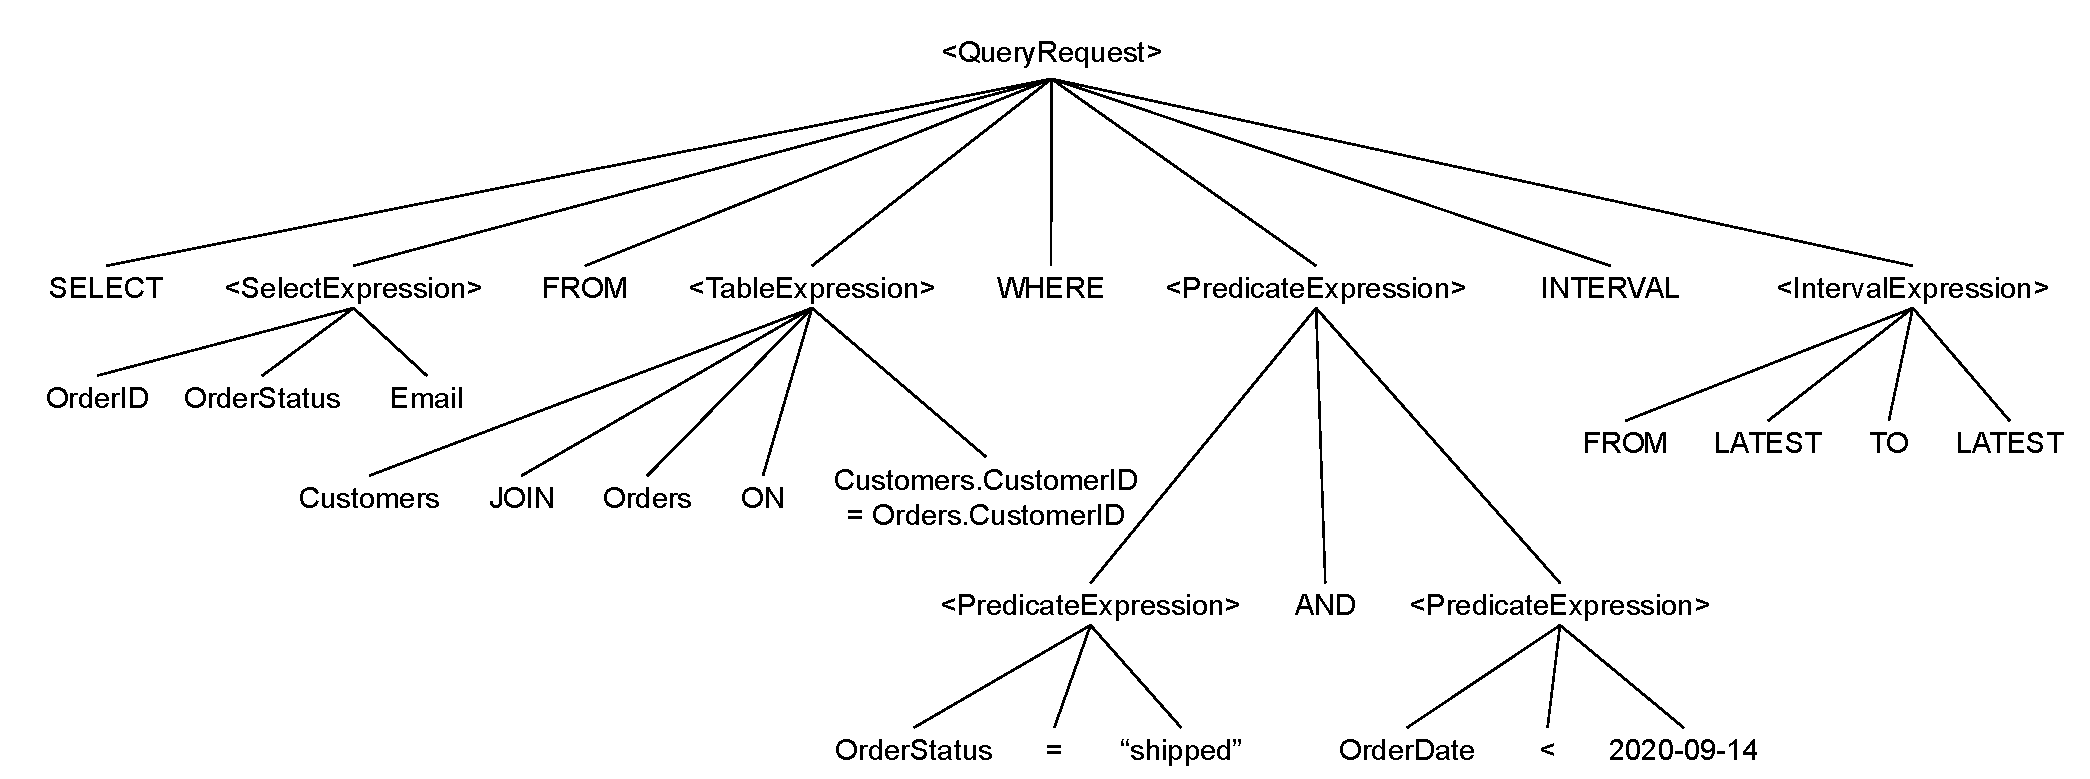
\includegraphics[width=\textwidth]{./figures/design_pattern/parse_tree.pdf}
  \caption{Query parse tree}
  \label{fig:parse_tree}
\end{figure}

The first step of a QPU's query processing function is to parse the given query from a string to a form that can be used
for query processing computations.
This form is a \textit{parse tree}.

A parse tree is constructed by applying the QPU query language's syntax rules to a given query string.
More specifically, a parse tree is composed to two types of nodes:

\begin{itemize}
  \item \textbf{Atoms}, which include keywords of the query language ($SELECT$, $FROM$ etc.),
  identifiers (such as table and attribute names), constants, operators and tokens.
  Atoms are leaf nodes of the parse tree.

  \item \textbf{Syntactic categories}, which are constructs built from atoms or other syntactic categories
  following the query language's syntax rules.
  Syntactic categories are internal nodes of the parse tree.
\end{itemize}

\noindent
For example, the parse tree for the query:
{\obeylines\obeyspaces
\texttt{
        SELECT OrderID, OrderStatus, Email
        FROM Customers JOIN Orders ON Customers.CustomerID = Orders.CustomerID
        WHERE OrderStatus != "shipped" AND OrderDate < 2020-09-14
        TIMESTAMP FROM LATEST TO LATEST
        }}
~ \\
\noindent
is depicted in Figure~\ref{fig:parse_tree}.

\subsubsection{Query processing capabilities tree}
\label{sec:qpc_tree}

In this section we present the \textit{query processing capabilities tree} (QPC tree).
The QPC tree represents the \textbf{set of all query parse trees that a QPU can process}.
Each QPU with downstream connections maintains a QPC tree for each of its downstream connections
(this consists the QPU's local graph view state).

The goal of the QPC tree is to represent the parse tree of all queries that a QPU can process.
The QPC tree is an extension of the query parse tree described in the previous section;
it uses an additional type of tree node, called \textbf{conjunction}.
Conjunction nodes represent the \textit{different potential sub-trees} of a syntactic category node.
Conjunction nodes essentially express the different branches of a syntax rule.

Figures~\ref{fig:qpt_corpus_driver_customers},~\ref{fig:qpt_corpus_driver_orders},~\ref{fig:qpt_filter_customers},~\ref{fig:qpt_filter_orders}, and~\ref{fig:qpt_join}
show the query processing capabilities trees for the QPUs in the ``customers - orders'' example.

\begin{figure}[t]
  \centering
    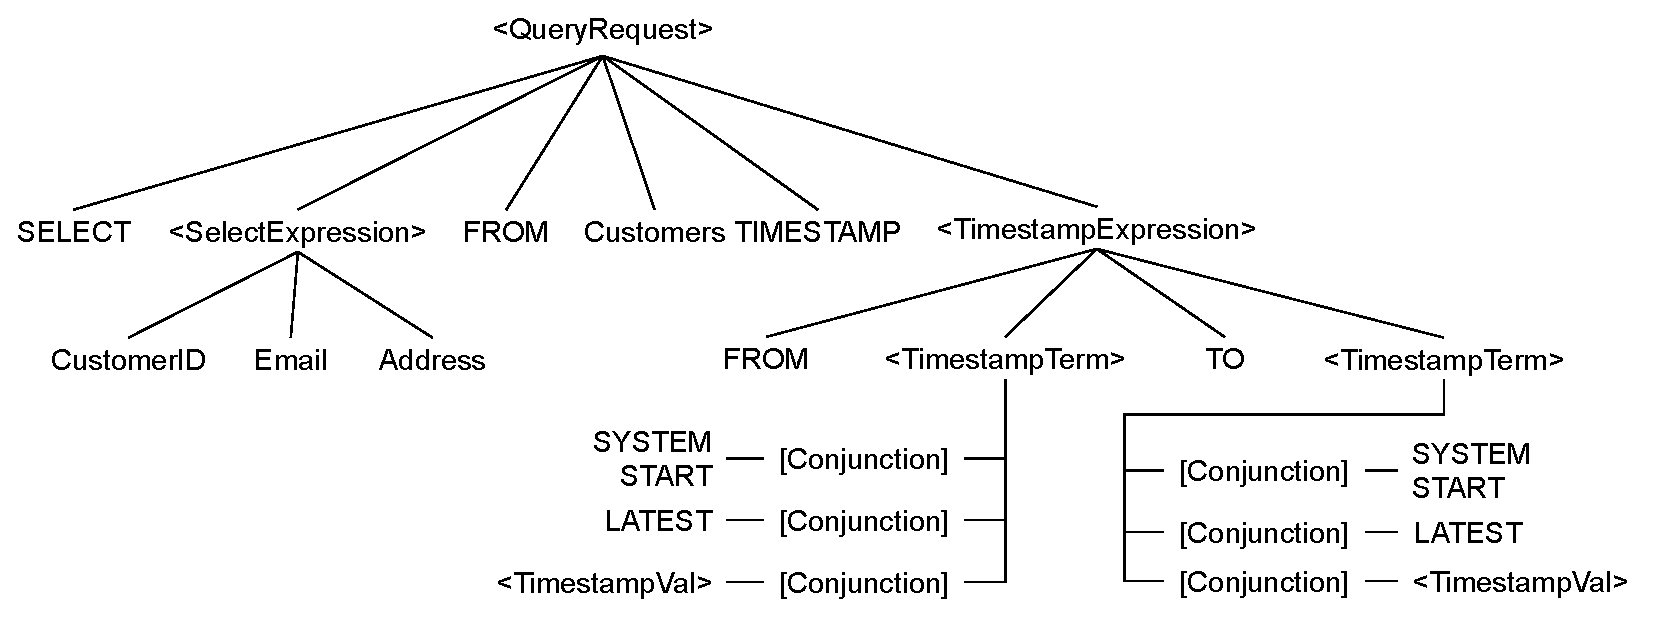
\includegraphics[width=\textwidth]{./figures/design_pattern/qpt_corpus_driver_customers.pdf}
  \caption{Query processing tree for $corpus$ $driver_1$}
  \label{fig:qpt_corpus_driver_customers}
\end{figure}

\begin{figure}[t]
  \centering
    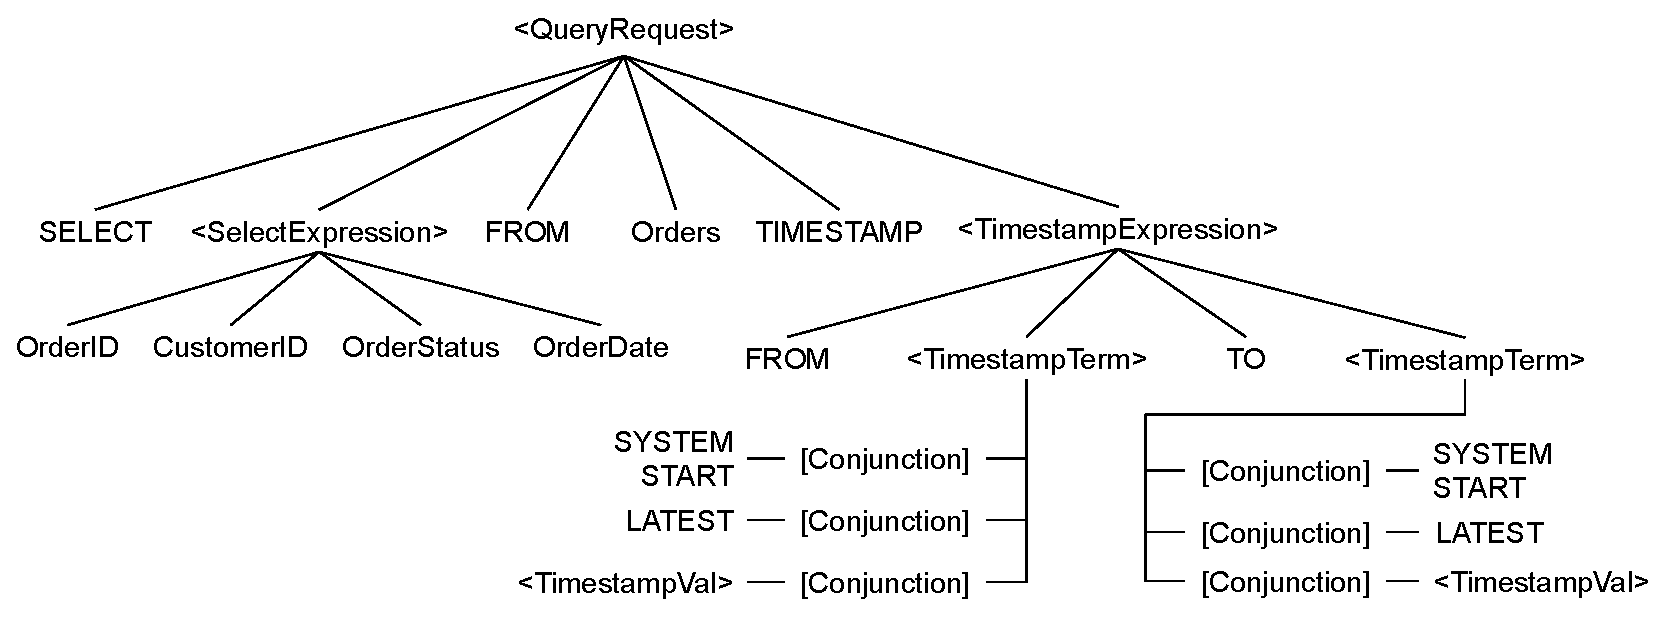
\includegraphics[width=\textwidth]{./figures/design_pattern/qpt_corpus_driver_orders.pdf}
  \caption{Query processing tree for $corpus$ $driver_2$}
  \label{fig:qpt_corpus_driver_orders}
\end{figure}

\begin{figure}[t]
  \centering
    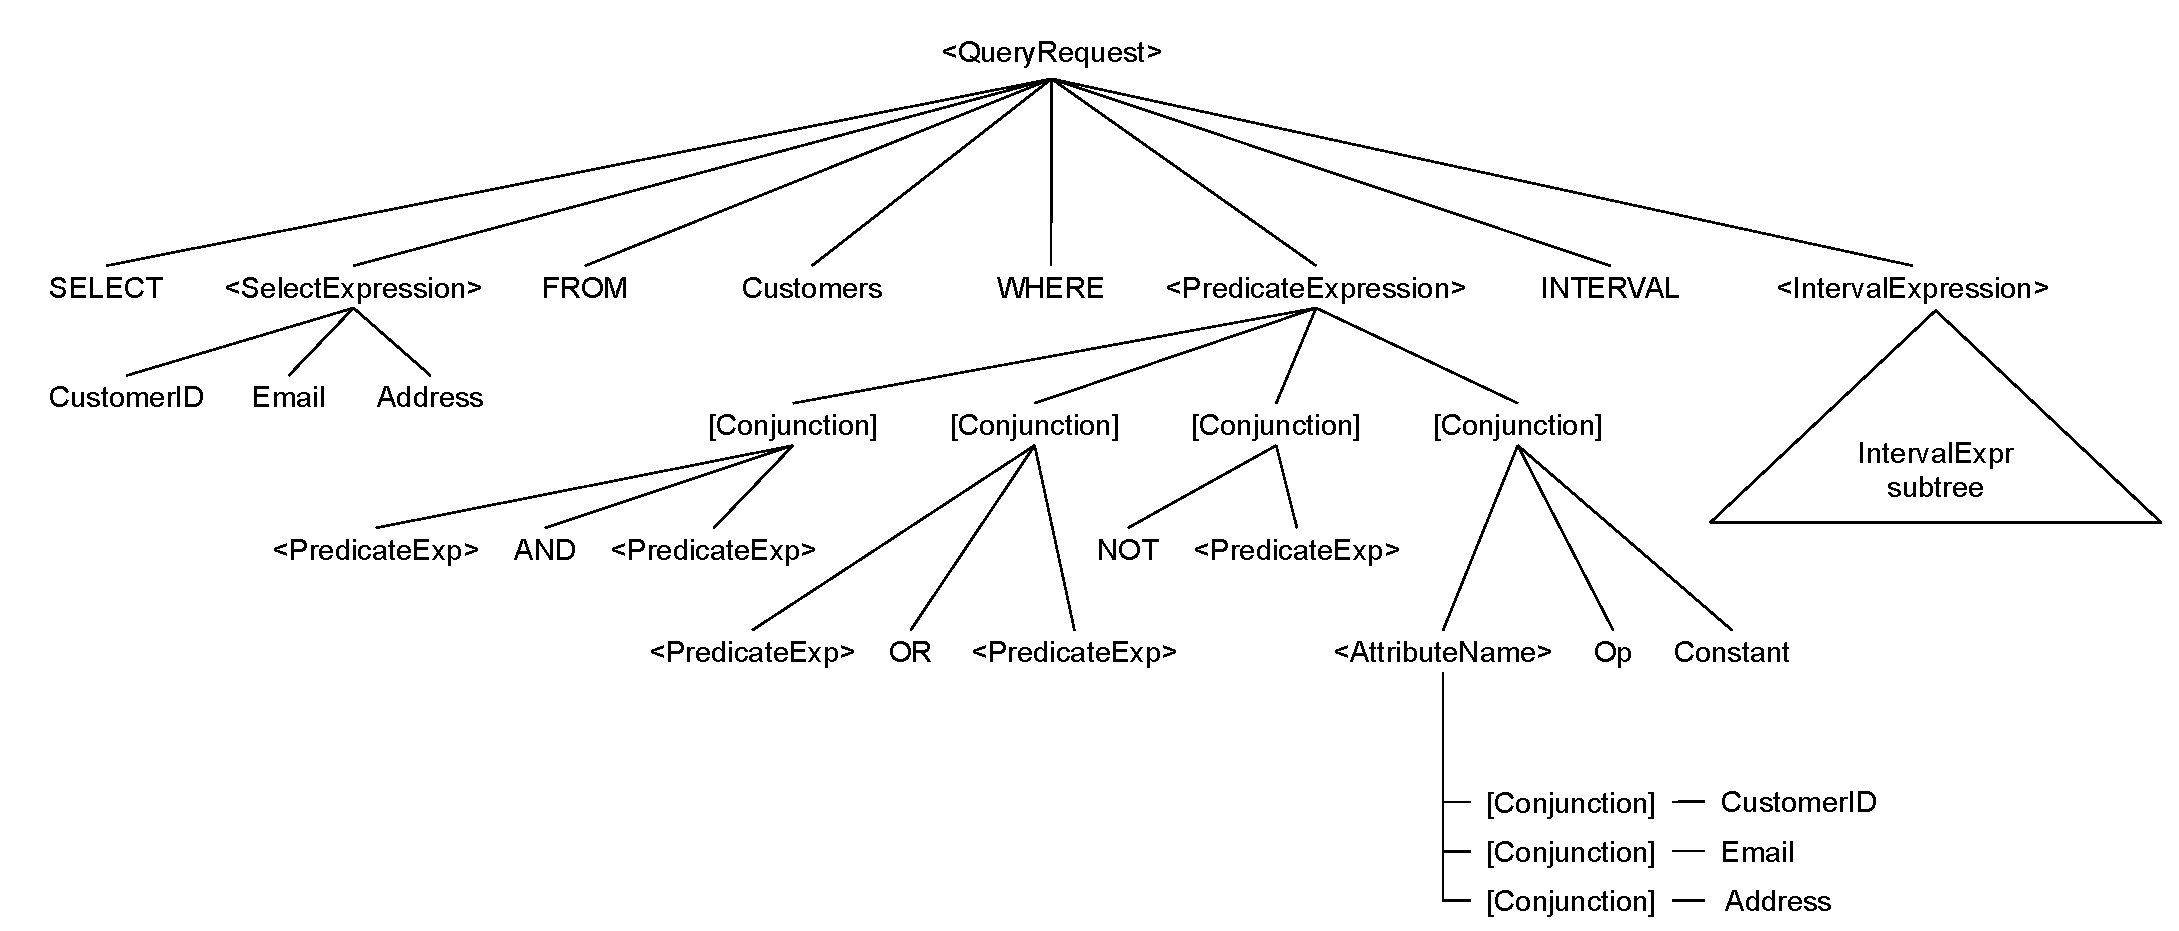
\includegraphics[width=\textwidth]{./figures/design_pattern/qpt_filter_customers.pdf}
  \caption{Query processing tree $filter_1$}
  \label{fig:qpt_filter_customers}
\end{figure}

\begin{figure}[t]
  \centering
    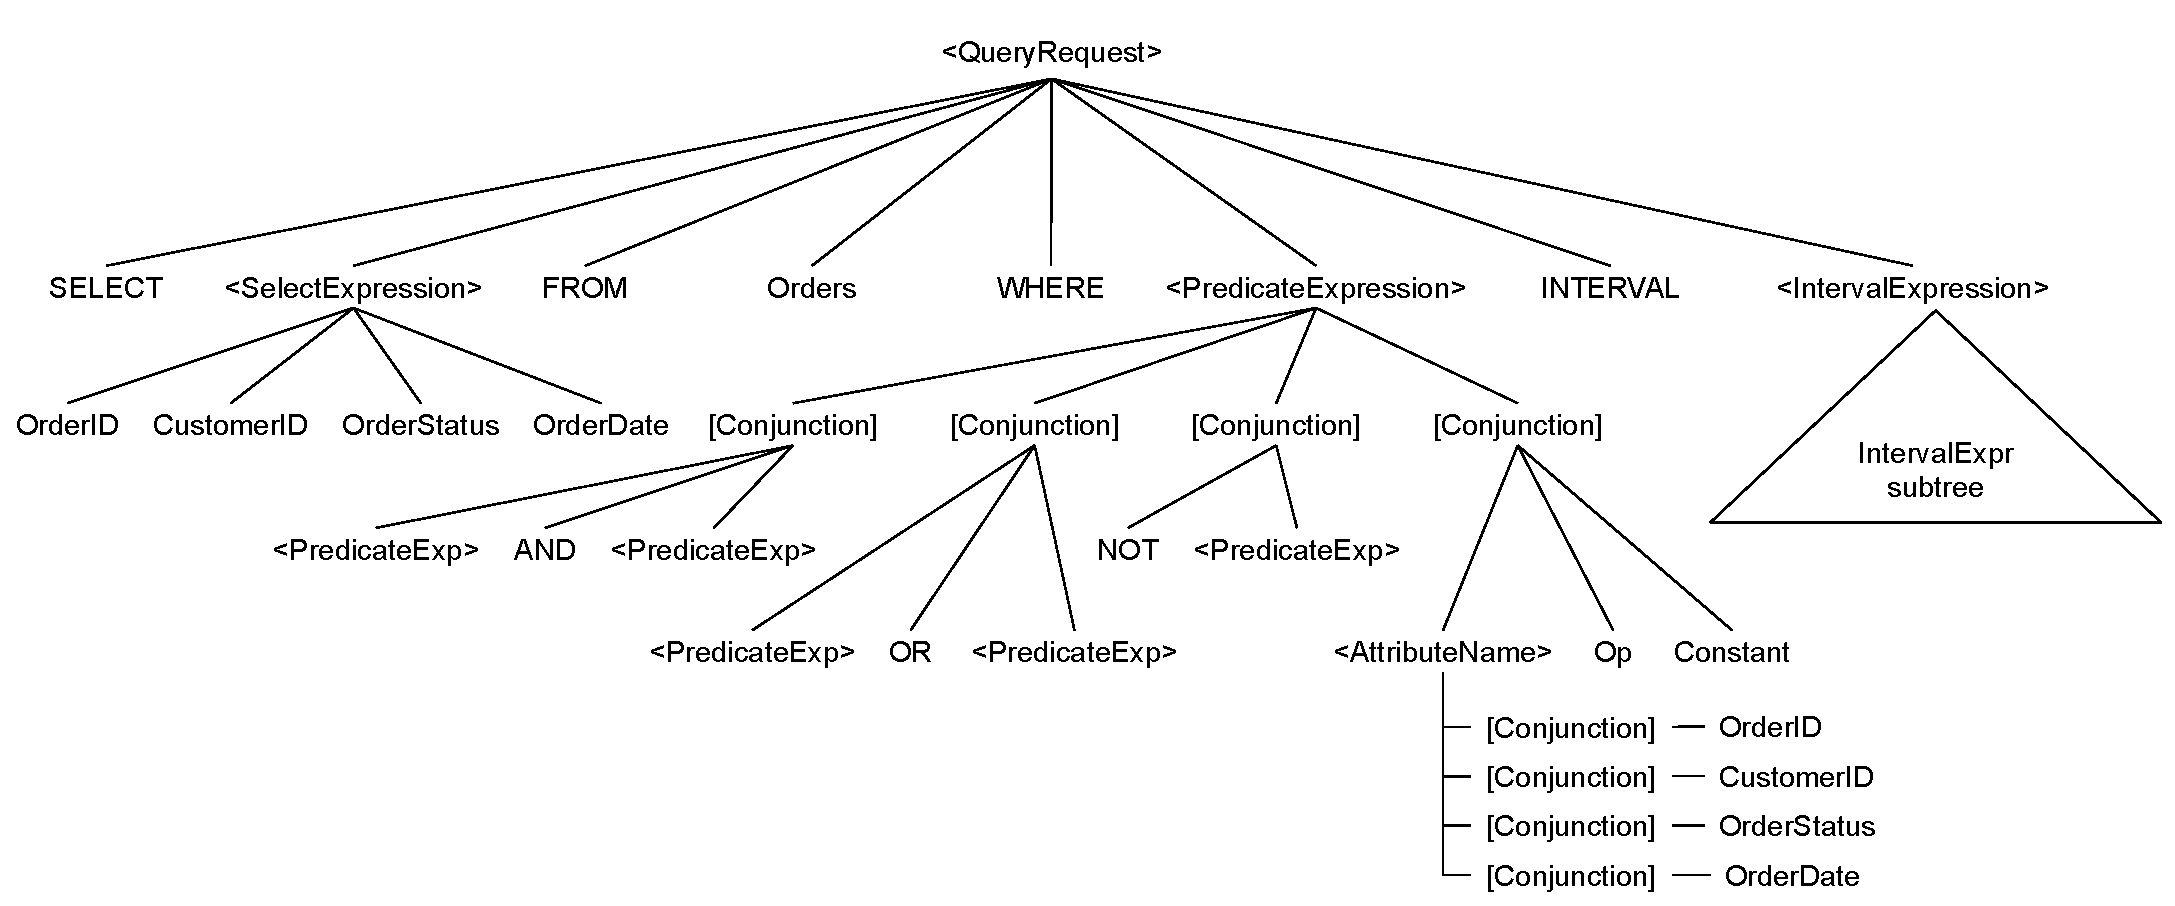
\includegraphics[width=\textwidth]{./figures/design_pattern/qpt_filter_orders.pdf}
  \caption{Query processing tree for $filter_2$}
  \label{fig:qpt_filter_orders}
\end{figure}

\begin{figure}[t]
  \centering
    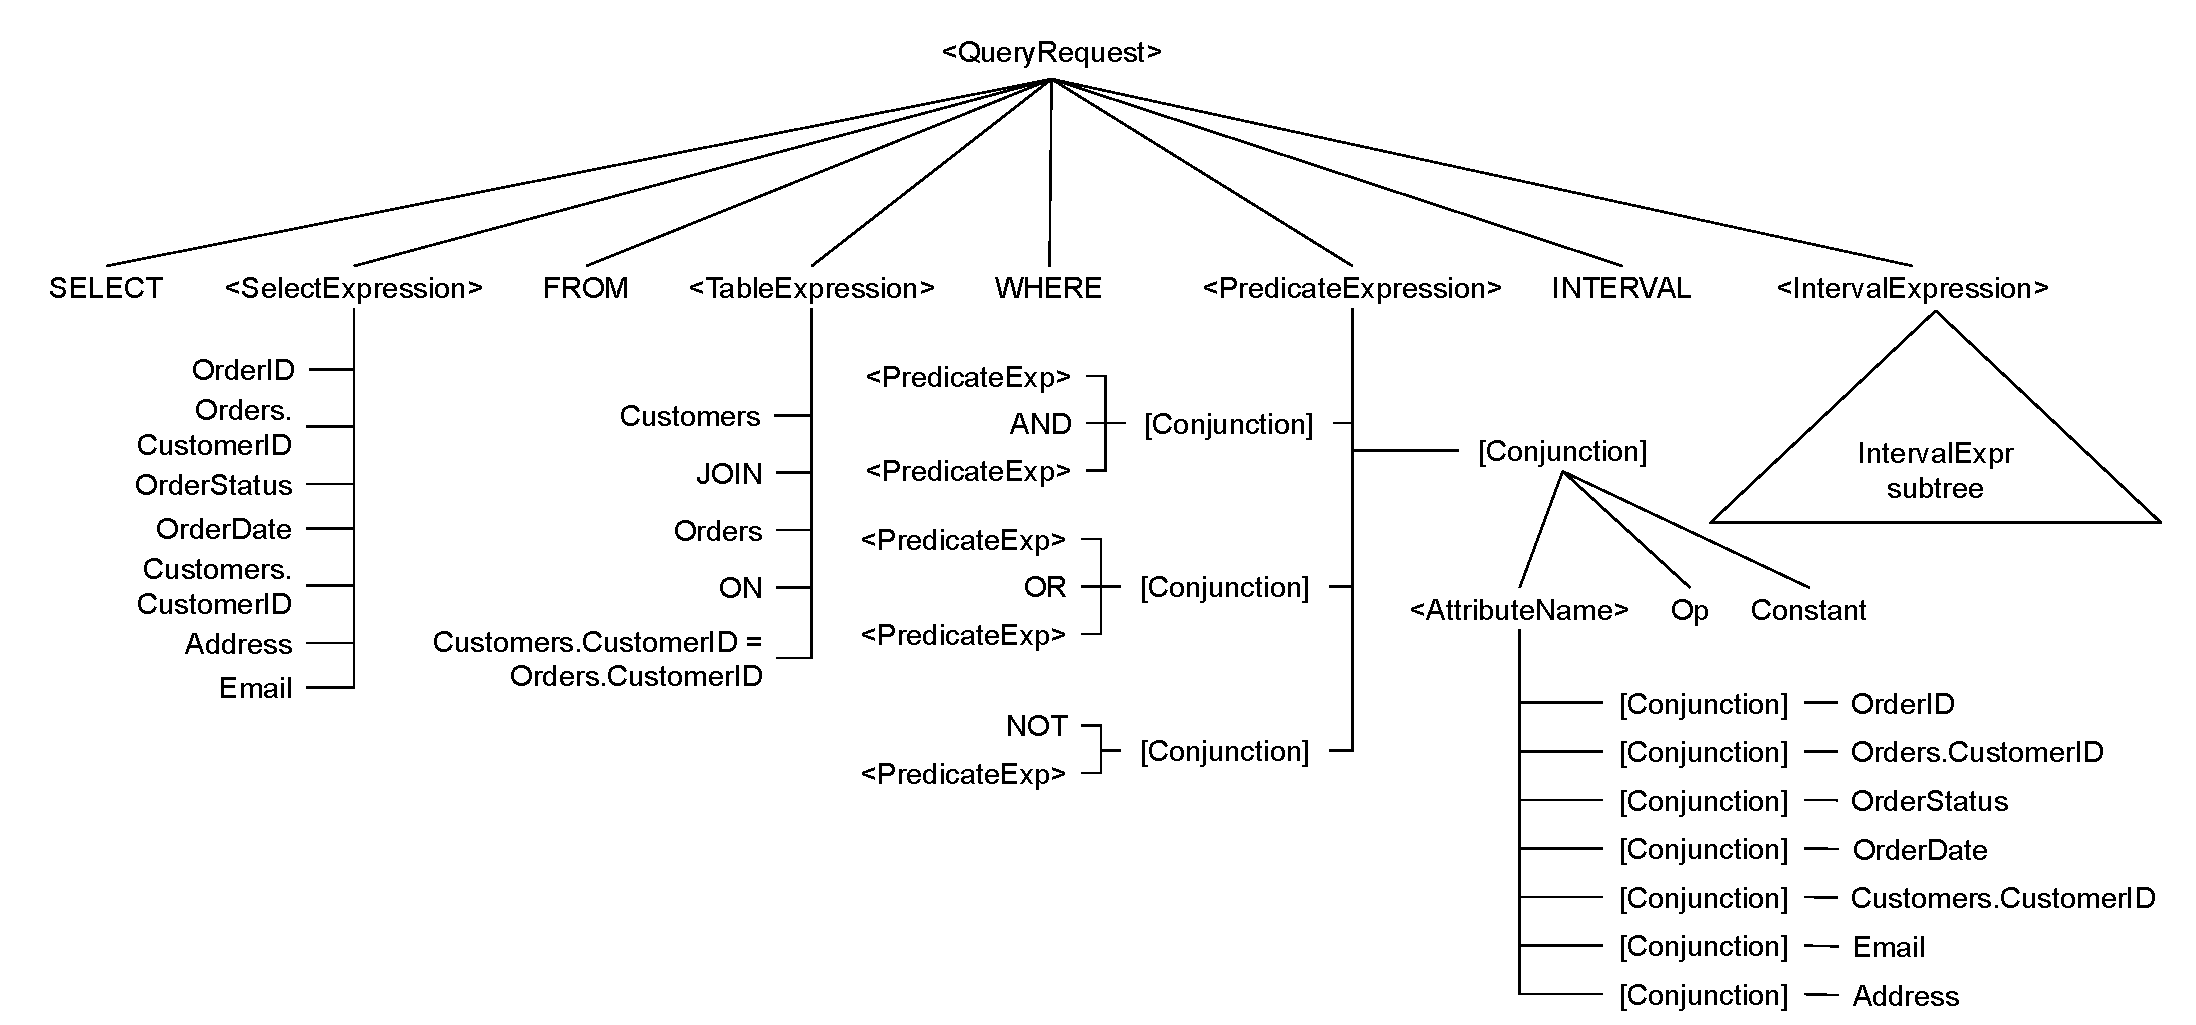
\includegraphics[width=\textwidth]{./figures/design_pattern/qpt_join.pdf}
  \caption{Query processing tree for $join$}
  \label{fig:qpt_join}
\end{figure}

QPU trees have two functionalities:
\begin{itemize}
  \item A query processing unit uses its own QPC tree in order to determine it can process a given query.
  More specifically, it checks it the query's parse is a \textbf{subtree} of the QPU's QPC tree,
  and, therefore, if the query's parse tree belongs in the set of queries represented by the QPU tree
  (algorithm~\ref{algo:can_process_query}).

  \item A query processing unit uses the QPC trees of its downstream connections in order to generate downstream queries.
  Given a query $q$ with parse tree $PT_q$, received a query processing unit $Q$ that has a downstream connections $Q_d$
  with QPC tree $QPCT_{Qd}$, the parse tree of the downstream query to be sent from $Q$ to $Q_d$ for $q$ is the
  \textbf{intersection} of $QPCT_{Qd}$ and $PT_q$
  (algorithm~\ref{algo:generate_downsrream}).
\end{itemize}

\begin{algorithm}
\caption{Algorithm for check if a query can be processed}
\label{algo:can_process_query}
\begin{algorithmic}
\Function{CanProcessQuery}{queryReq, QPCTree}
\State queryParseTree = parse queryReq
\State \Return {isSubTree(QPCTree, queryReq)gs}
\EndFunction
\end{algorithmic}
\end{algorithm}

\begin{algorithm}
\caption{Algorithm for generating downstream queries}
\label{algo:generate_downsrream}
\begin{algorithmic}
\Function{GenerateDownstreamQuery}{queryReq, downstreamConn}
\State queryParseTree = parse queryReq
\State qpcTree = get QPC tree of downstreamConn
\State downStreamQueryParseTree = intersection(qpcTree, queryParseTree)
\State downStreamQueryReq = generate query from parse tree
\State \Return downStreamQueryReq
\EndFunction
\end{algorithmic}
\end{algorithm}

% \subsubsection{Ordering guarantees}

% Providing ordering guarantees is based on two mechanisms:
% For a given query $q$:
% \begin{itemize}
%   \item Leaf nodes (corpus driver and derived state classes) generate ordered output streams,
%   based on the ordering specified by $q$.

%   \item Relational operator classes ensure that they \textit{preserve} the ordering of
%   their input stream at their output stream.
% \end{itemize}

% //// Outline ////

% Illustrate using example:
% {\obeylines\obeyspaces
% \texttt{
%         SELECT OrderID, OrderStatus, Email, OrderDate
%         FROM Customers JOIN Orders ON Customers.CustomerID = Orders.CustomerID
%         WHERE OrderStatus = "Processing"
%         TIMESTAMP FROM LATEST TO LATEST
%         ORDER BY OrderDate
%         }}

% \begin{itemize}
%   \item Corpus driver for Orders Table generates output stream ordered by OrderDate
%   \item Filter table keeps only records for which OrderStatus = ``Processing''; this preserves order
%   \item Join uses input from Orders table as ``ordering guide''; this ensures that output is ordered by
%   by OrderDate
% \end{itemize}

% \medskip
% \noindent
% More details on how QPUs preserve ordering semantics:
% \begin{itemize}
%   \item Trivial for QPU's with one input stream
%   \item For QPUs that merge more than one input streams (for example a partition manager), since each input stream
%   is ordered, the ``mergesort'' approach can be used.
%   \item Joins can preserve ordering by using the ``ordered'' input stream as a guide.
%   \item Aggregators (TODO)
% \end{itemize}

% //// Outline ////

\section{Discussion}

\noindent
\textbf{On the query processing unit semantics}.

\noindent
Representing a relational algebra query execution as a dataflow computation performed by a DAG of operators is a common
technique in the state of the art \cite{cockroachdb:distsql}.
However this technique is focused on expressing relational algebra expressions.
It does not include the incremental maintenance of derived state, or ``systems'' functionalities such as load balancing
and the management of access to partitioned state.

Our first insight is that these three types of functionalities can be encapsulated by components with microservice semantics:
exposing their functionality through an invocation of an interface.
For components that encapsulate derived state components this is already the case, as for example indexes expose a
Lookup()/Get() API.
This can be extended to components that encapsulate relational operators and ``routing'' functionalities.

Moreover, this interface can be common for all three types of components:
\begin{itemize}
  \item An index lookup can be expressed as a query statement for the indexed attribute.
  \item Reading from a materialized view can be expressed by the query that consists the view's definition.
  \item Initiating the functionality of a relational operator can be expressed by a query that represents the
  operator's functionality.
  For example a join operator can be initiated with a ``SELECT - FROM - JOIN'' query.
\end{itemize}

A result of this is that  individual components do not support the complete query language.
Instead, each performs a basic operation, based on its functionality.
It is through \textit{composition} that more complex query processing functionalities can be achieved.

Composition is achieved using the microservice semantics:
a component can invoke the interface of other components in order to obtain partial results needed for its operation.
In addition, this characteristic achieves modularity.
Because communication between components is performed through well-defined interfaces,
component placement is orthogonal to the system's functionality, and components can be flexibly placed across the system.

However, an additional requirement exists for indexes and materialized views:
a mechanism for keep these structures up-to-date with the corpus by performing incremental updates.
Our second insight is that this mechanism can be expressed as an input stream of update events.
Therefore, the input stream semantics of relational operators can be generalized to also express incremental updates to derived state.

However, streams that represent query results contain data items' \textit{state} as their records,
while streams that represent corpus contain update events.
Our third insight is that these two types of records can be unified by structuring stream records as
\textit{deltas}.

Finally, the above insight are combined by specifying tha the response to the invocation of a components interface is a stream.
As a result, the query processing unit computation model combines elements from microservice architectures and stream processing systems.
Similar to stream processing systems,
query processing units operate on input streams, and either perform transformations on those stream creating an output
stream, or uses to incrementally update its state.
Similar to microservices architectures, a stream is initiated as a response to a \textit{service request}.

\medskip
\noindent
\textbf{On QPU-based query processing systems and ad-hoc queries}.

\noindent
The goal of the QPU-based design pattern is to enable \textit{workload-driven design}.
A QPU graph is designed based a predefined set of query patterns.
As a result, a QPU graph does not support any ad-hoc query,
but rather \textit{the set of queries it has been designed for}.
More specifically, as described in section~\ref{sec:qpc_tree}, a QPU graph supports the set of queries represent by the QPC trees of its root nodes.
Supporting additional query patterns, not supported by a certain QPU graph requires designing and deploying a
new QPU graph.

% Given $q$, the query processing function of a QPU $Q$ at the root of the QPU graph sends query request to some its
% downstream connection, in order to initialize input stream required for processing the query.
% Upon receiving a query request from $Q$, each of its downstream connection performs the same process.
% In that way, query requests are propagated downwards through the QPU graph, creating a \textit{query execution sub-graph}
% composed of the QPUs that participate in the processing of $q$.

% As query requests requests are propagated downwards, expanding the $q$'s execution sub-graph, eventually some QPUs can
% process their queries without sending further query requests downwards.
% This occurs in corpus driver and derived state QPUs.
% The leaves of this sub-graph are QPU that can process 
% This includes corpus driver QPUs, and derived state QPUs.
% These QPUs produce output streams that are then processed as input stream at \textit{upstream QPUs}.

% Progressively, each non-leaf QPU in the query sub-graph receives an input stream for each query request sent,
% and produces it self an output 


% We describe how a QPU graph processes a given query using the example of Figure~\ref{fig:qpu_graph_emergent_properties}.

% Consider the query:
% {\obeylines\obeyspaces
% \texttt{Q = SELECT CustomerName, CustomerEmail, OrderID
%         ~~~~FROM Customers
%         ~~~~INNER JOIN Orders ON Customers.OrderID = Orders.OrderID
%         ~~~~WHERE Orders.OrderDate >= 2020-08-20 AND Orders.OrderDate < 2020-09-02
%         ~~~~TIMESTAMP FROM LATEST TO LATEST
%         }}

% - queries / control messages flow downwards.
% - responses flow upwards through the sub-graph defined by the queries
% - (each query establishes a sub-graph - actually a tree - to be used by that particular query);
% - Updates (independently) also flow upwards

% As described in the previous sections, query processing units can collaborate by invoking the query API of one another.
% QPUs can be composed in DAG hierarchies in which parent units can invoke the query API of their child units.
% Query responses for both snapshot and persistent queries are streams of results.
% Communication between QPUs thus uses a combination of the remote procedural call model (query API invocations) and the stream-processing model (query responses).

% Clients perform queries by invoking the query API of units at root nodes of the graph.
% Once a QPU receives a query, it determines whether it can directly process it, for example by performing lookups at its indexing structures,
% and if that is the case it responds with the query result.
% In case the query processing computation requires partial query results from its child units, the unit invokes the query API of those units with the appropriate sub-queries.
% Sub-query results are received and processed through the unit's callback function.

% This process is recursively performed at each query processing unit.

% Therefore, the computation that runs in QPU a graph can be modeled as a bidirectional data-flow computation.
% Queries flow downwards through the graph, are incrementally split into sub-queries, and processed across the graph.
% Sub-query results flow back upwards, are incrementally processed, and eventually produce the results to the initial query.

% The same computation model is used for index maintenance.
% We have extended the query interface semantics so that the query API can be used to subscribe to notifications for corpus updates, and query results can encode these updates.
% Using this mechanism, units with indexing functionalities can subscribe to corpus updates by invoking the query API of QPUs that provide this functionality.
% We describe this mechanism in more detail in Section \ref{subsec:query_classes}.


% The QPU graph runs a distributed bidirectional data-flow computation.

% A client performs a query $Q_c$ by invoking the query API of a query processing unit at the root of the graph.
% As described in Section~\ref{subsec:qpu}, the QPUs query processing computation can read from the unit's state,
% or perform downstream queries to QPUs at its child nodes.

% When a downstream query is performed, this process is recursively executed at each unit whose query API is invoked.
% Though this mechanism, $Q_c$ is incrementally transformed to sub-queries which flow downwards through the QPU graph,
% invoking computations at different nodes.
% Sub-query results are returned through the QPU streams established from query API invocations, and flow upwards
% through the graph.
% These results are incrementally processed, potentially updating the state of different QPUs, and eventually
% produce the initial query results, which are returned to the client.

% \section{QPU Composition: Constructing QPU-based query engines}
% Here, describe how query engines are constructed using instances of QPU classes.

% A query engine is a directed acyclic graph (why?) with QPUs as nodes.

% Describe the QPU-specific topology properties that the graph must satisfy in
% order to be functional:
% \begin{itemize}
%   \item All leaves must be QPUs of the datastore driver class.
%   Also, datastore driver QPUs cannot be nodes other than leaves.
%   \item TODO
% \end{itemize}

% \section{Computation Model}
% Describe the bidirectional data-flow computation.
% \begin{itemize}
%   \item Control messages (queries) flow downwards.
%   \item Responses flow upwards through the sub-graph defined by the control
%   (each query establishes a sub-graph - actually a tree - to be used by that
%   particular query);
%   \item Updates (independently) also flow upwards.
% \end{itemize}


% % \section{The consistency guarantees of QPU-based query engines}
% % TODO: What mechanism are needed so that QPUs can guarantee internal consistency?
% % What about session consistency guarantees?



% % It is known that query execution can be represented as a tree.
% % Base data are at the tree's leaves, tree nodes are relational operator such
% % as filter, joins and aggregations, and query result are at the root of the tree.
% % Each operator receives an input stream of records, performs a transformation on the, and emits a output stream of record.
% % This results to a data-flow computation in which data items flow upwards through the tree and are progressively transformed
% % to the query execution results.

% % Computation tasks vs architecture components

% % Our approach is based on three simple insights:
% % \begin{itemize}
% %     \item \textbf{Index-based distributed query processing is composed of basic, primitive tasks.}
% %     The most simple query engine design is a component that scans the corpus dataset and selects the data items which match a given query.
% %     When queries for certain attributes are frequent or require low response time, secondary indexes can be materialized for those attributes.
% %     Even when indexes are partitioned and distributed across the system for scalability, the basic components of an indexing system remains the same: index data structures that collaborate through appropriate index maintenance and query processing protocols to implement distributed indexes.
% %     Additional query processing functionalities such as multi-attribute queries, joins or federated queries across multiple corpus can be implemented using operators that build on top of these components.
% %     Finally, caching can be used to further improve response time for certain queries.

% %     \item \textbf{Primitive query processing tasks can be encapsulated by a common query processing component model.}
% %     Each of the described tasks can be encapsulated by a query processing component model with two properties: an API for responding to queries, and a callback function.
% %     For example, index data structures in general implement three basic functions: LOOKUP, INSERT, DELETE.
% %     The query API can encapsulate the LOOKUP function, while the callback function can express the task of index maintenance, receiving corpus updates and updating the index accordingly, and therefore encapsulate INSERT and DELETE.
% %     As another example, a cache on top of an index structure should be able to respond to the same queries as the underlying index, and therefore can be encapsulated by a query processing component with the same query API.
% %     Similarly, its callback function can express the task of receiving query results in case of a cache miss, and updating the cache.
% %     This concept can be generalized to represent other query processing components including bloom filters, materialized views, and streaming operators.

% %     \item \textbf{Query processing components need to cooperate to implement complex query processing tasks.}
% %     As an example, a caching component requires the ability to forward queries to other components, such as indexes, when cache misses occur.
% %     Similarly, a distributed indexing system, in which indexes are partitioned and distributed across system nodes, can be implemented using indexing components with the help of an additional component responsible for implementing a partitioned LOOKUP operation, by collecting and aggregating partial LOOKUP results.
% % \end{itemize}

% % Based on these observations, we introduce a query processing component model, called the \textit{Query Processing Unit} (QPU).
% % We have designed a generic query API and callback function interface with the aim of encapsulating multiple different query processing components.
% % Query processing units may have internal state for facilitating query processing, or be stateless.
% % Additionally, QPUs have the ability to invoke the query API of one another, and thus interoperate for query processing.


\bibliographystyle{plainnat}
\bibliography{refs}